\documentclass[12pt,a4paper]{article}

% Pacotes essenciais
\usepackage[utf8]{inputenc}
\usepackage[T1]{fontenc}
\usepackage[portuguese]{babel}
\usepackage{amsmath,amsfonts,amssymb}
\usepackage{graphicx}
\usepackage[a4paper,margin=2cm]{geometry}
\usepackage{booktabs}
\usepackage{float}
\usepackage{caption}
\usepackage{hyperref}

\graphicspath{{resultados/}}
\newcommand{\R}{\mathbb{R}}

% Título e cabeçalho
\title{{\footnotesize Universidade Federal de Minas Gerais\\Escola de Engenharia\\ELE077 Otimização Não Linear\\} \vspace{5mm} Trabalho Computacional I}

% Autores do trabalho
\author{Luisa Marques Laboissiere \and Talvani de Souza Barbosa}
\date{4 de novembro de 2026}

\begin{document}

\maketitle

\section*{Introdução}

Este relatório resolve os quatro problemas de otimização não linear irrestrita do Trabalho Computacional~I. Para cada problema, a função-objetivo é analisada quanto a diferenciabilidade, convexidade, modalidade e dimensão; a partir dessa análise escolhe-se o método mais adequado, cujos resultados são apresentados e discutidos.

Todos os métodos foram executados com \texttt{scipy.optimize.minimize} (Python 3.12, SciPy 1.18, NumPy 2.5, Matplotlib 3.11). Cada questão corresponde a um script (\texttt{questao1.py} a \texttt{questao4.py}); os resultados numéricos são gravados em \texttt{resultados/questaoN/resultados.json} e as figuras na mesma pasta. A Tabela~\ref{tab:resumo} resume as escolhas.

\begin{table}[H]
\centering
\caption{Resumo das características de cada problema e do método escolhido.}
\label{tab:resumo}
\begin{tabular}{@{}cccccc@{}}
\toprule
Problema & Variáveis & Diferenciável & Convexa & Método & Derivadas usadas \\
\midrule
1 & 3    & Sim ($x\neq 0$) & Não  & BFGS          & Gradiente analítico \\
2 & 1024 & Sim (via $\epsilon$) & Sim & Gradientes Conjugados & Gradiente analítico \\
3 & 2    & Não             & Não (em $p$) & Nelder--Mead & Nenhuma \\
4 & 2    & Sim             & Estritamente & Newton & Gradiente e Hessiana \\
\bottomrule
\end{tabular}
\end{table}

% =====================================================================
\section{Problema 1 --- Frequência natural fundamental}

\subsection{Análise da função-objetivo}

A função a minimizar é o quociente de Rayleigh
\begin{equation}
R(\mathbf{x}) = \frac{\mathbf{x}^T\mathbf{K}\mathbf{x}}{\mathbf{x}^T\mathbf{M}\mathbf{x}}, \qquad \mathbf{x}\in\R^3\setminus\{\mathbf{0}\},
\end{equation}
com $\mathbf{M}=\mathbf{I}$ e $\mathbf{K}$ dada no enunciado. Suas principais características são:

\begin{itemize}
  \item \textbf{Diferenciabilidade.} $R$ é infinitamente diferenciável em todo ponto com $\mathbf{x}\neq\mathbf{0}$, e o gradiente tem forma fechada simples:
  \begin{equation}
  \nabla R(\mathbf{x}) = \frac{2\left(\mathbf{K}\mathbf{x} - R(\mathbf{x})\,\mathbf{M}\mathbf{x}\right)}{\mathbf{x}^T\mathbf{M}\mathbf{x}}.
  \end{equation}
  \item \textbf{Invariância de escala.} $R(\alpha\mathbf{x}) = R(\mathbf{x})$ para todo $\alpha\neq 0$. Portanto o minimizador não é um ponto isolado, mas uma reta (sem a origem): só a \emph{direção} de $\mathbf{x}^*$ é determinada, não sua magnitude nem seu sinal.
  \item \textbf{Pontos estacionários.} $\nabla R(\mathbf{x})=\mathbf{0}$ equivale a $\mathbf{K}\mathbf{x}=R(\mathbf{x})\mathbf{M}\mathbf{x}$, isto é, os pontos estacionários são exatamente os autovetores do problema generalizado $(\mathbf{K},\mathbf{M})$, e o valor de $R$ em cada um é o autovalor correspondente. Com $\lambda_1<\lambda_2<\lambda_3$, o primeiro autovetor é mínimo global, o segundo é ponto de sela e o terceiro é máximo global.
  \item \textbf{Convexidade e modalidade.} $R$ não é convexa (possui ponto de sela e máximo), mas todo mínimo local é global: não existem mínimos locais espúrios.
  \item \textbf{Hessiana.} No ótimo, $\nabla^2 R(\mathbf{x}^*) = 2(\mathbf{K}-\lambda_1\mathbf{M})/(\mathbf{x}^{*T}\mathbf{M}\mathbf{x}^*)$, que é semidefinida positiva e \emph{singular} (anula-se na direção do próprio $\mathbf{x}^*$, consequência da invariância de escala). Fora do ótimo, a Hessiana pode ser indefinida.
\end{itemize}

Como $R$ só depende da direção de $\mathbf{x}$, é possível visualizar a função fixando $x_3=1$: qualquer vetor com $x_3\neq 0$ pode ser reescalado para esse plano sem alterar $R$. A Figura~\ref{fig:q1} (esquerda) mostra as curvas de nível de $R(x_1,x_2,1)$ com os três autovetores marcados, evidenciando o vale do mínimo, o ponto de sela e o máximo.

\subsection{Escolha do método: BFGS}

\begin{itemize}
  \item A função é suave e o gradiente analítico é barato, logo um método baseado em gradiente é natural; métodos de ordem zero (como Nelder--Mead) desperdiçariam essa informação.
  \item O \textbf{método de Newton} não é adequado: a Hessiana é singular no ótimo e pode ser indefinida em outros pontos, de modo que o passo de Newton pode não estar definido ou não ser direção de descida.
  \item O \textbf{BFGS} constrói uma aproximação da Hessiana que se mantém definida positiva, garantindo direções de descida, e converge de forma superlinear, muito mais rápido que o gradiente descendente.
  \item A dimensão é pequena ($n=3$), de modo que o custo de armazenar e atualizar a matriz $3\times3$ do BFGS é desprezível.
\end{itemize}

\newpage
\subsection{Resultados}

Utilizou-se \texttt{method='BFGS'} com o gradiente analítico, ponto inicial $\mathbf{x}_0=(1,1,1)$ e tolerância \texttt{gtol}$=10^{-10}$. A Tabela~\ref{tab:q1} resume os resultados.

\begin{table}[H]
\centering
\caption{Resultados do Problema 1 (BFGS).}
\label{tab:q1}
\begin{tabular}{@{}ll@{}}
\toprule
Grandeza & Valor \\
\midrule
$\mathbf{x}^*$ & $(0{,}6084;\ 1{,}0962;\ 1{,}3670)$ \\
$\mathbf{x}^*/x_3^*$ & $(0{,}4450;\ 0{,}8019;\ 1)$ \\
$R(\mathbf{x}^*) = \omega_1^2$ & $0{,}198062264195$ \\
$\omega_1$ & $0{,}44504$ rad/s \\
Iterações & 7 \\
Avaliações de $f$ / de $\nabla f$ & 8 / 8 \\
$|R(\mathbf{x}^*)-\lambda_{\min}(\mathbf{K})|$ & $1{,}9\times10^{-16}$ \\
Erro de direção em relação ao autovetor & $2{,}2\times10^{-12}$ \\
$\|\nabla R(\mathbf{x}^*)\|$ & $4{,}3\times10^{-12}$ \\
\bottomrule
\end{tabular}
\end{table}

\begin{figure}[H]
\centering
\begin{minipage}{0.49\textwidth}\centering
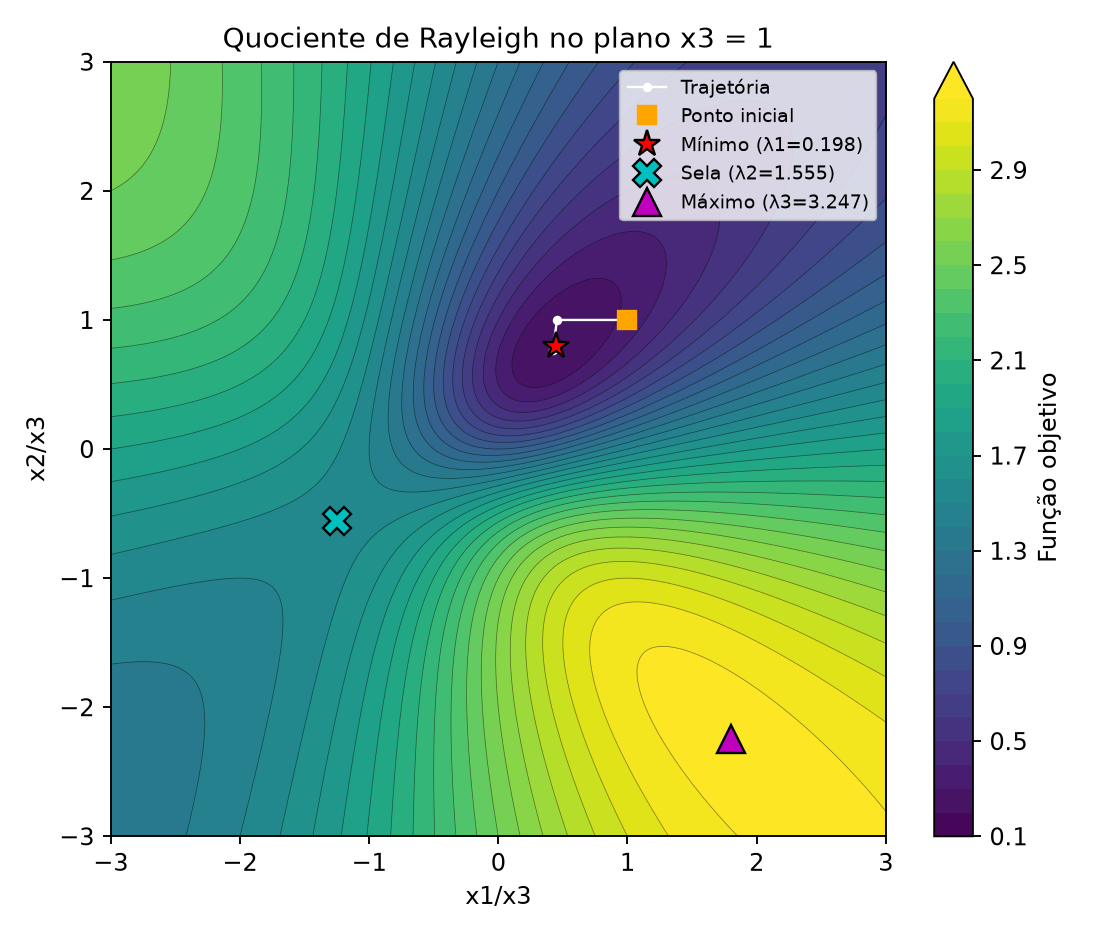
\includegraphics[width=\linewidth]{questao1/curvas_nivel.png}
\end{minipage}\hfill
\begin{minipage}{0.49\textwidth}\centering
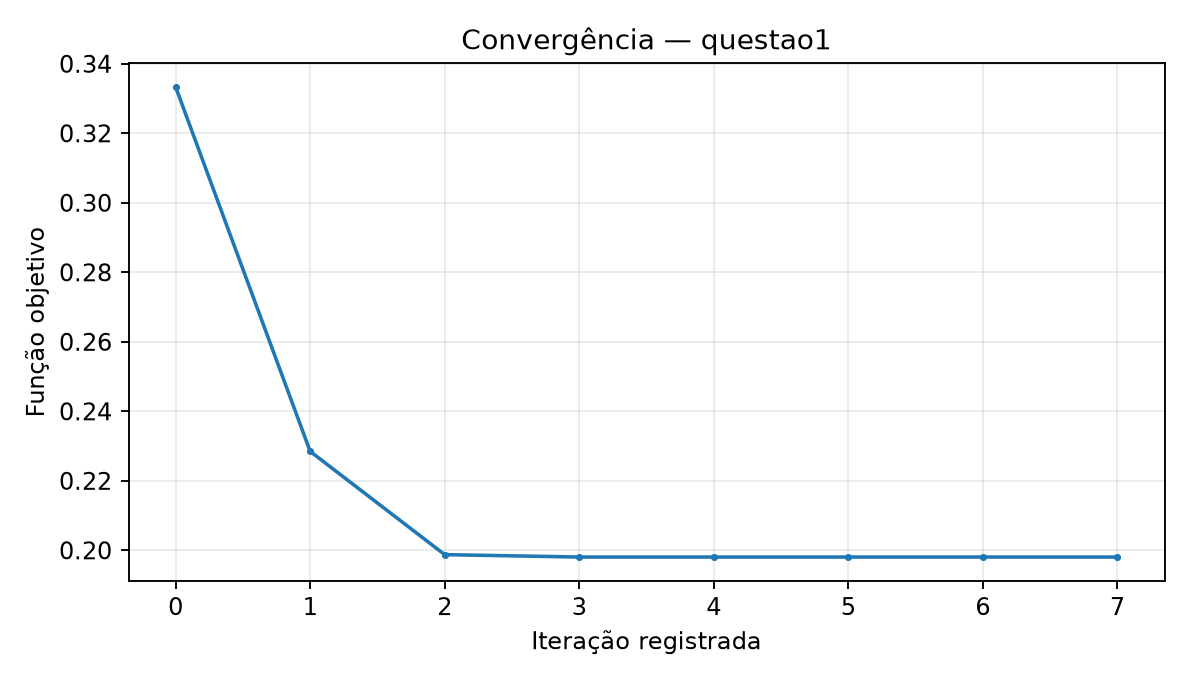
\includegraphics[width=\linewidth]{questao1/convergencia.png}
\end{minipage}
\caption{Problema 1. Esquerda: curvas de nível de $R$ no plano $x_3=1$, com a trajetória do BFGS projetada e os três autovetores de $\mathbf{K}$. Direita: valor de $R$ por iteração.}
\label{fig:q1}
\end{figure}

\subsection{Discussão}

O BFGS encontrou $\omega_1^2 = 0{,}198062$, que coincide com o menor autovalor de $\mathbf{K}$ calculado por \texttt{numpy.linalg.eigh} até a precisão de máquina, resultando em uma frequência natural fundamental $\omega_1 \approx 0{,}445$~rad/s. O valor também concorda com a expressão fechada $\lambda_1 = 2-2\cos(\pi/7) \approx 0{,}198062$ para esta matriz tridiagonal. A direção encontrada coincide com o primeiro autovetor (erro de $2\times10^{-12}$), e o resíduo $\|\mathbf{K}\mathbf{v}-R\,\mathbf{M}\mathbf{v}\|$ é da ordem de $4\times10^{-12}$.

A convergência foi superlinear: o erro $R(\mathbf{x}_k)-\lambda_1$ passou de $1{,}4\times10^{-1}$ para $3\times10^{-2}$, $7\times10^{-4}$, $10^{-6}$ e $6\times10^{-11}$ em iterações sucessivas, totalizando 7 iterações e 8 avaliações de função e gradiente. Na Figura~\ref{fig:q1} vê-se que a trajetória vai diretamente para o vale do mínimo, sem passar perto do ponto de sela.

A magnitude de $\mathbf{x}^*$ obtida ($\|\mathbf{x}^*\|\approx1{,}85$) é arbitrária: ela depende apenas do ponto inicial, pois o otimizador para em algum ponto da reta de minimizadores. Fisicamente, $\mathbf{x}^*$ é o \emph{modo de vibração} fundamental: as três massas se deslocam no mesmo sentido, com amplitudes crescentes da massa 1 para a massa 3 (razão $0{,}445 : 0{,}802 : 1$).

% =====================================================================
\section{Problema 2 --- Restauração de imagem por variação total}

\subsection{Análise da função-objetivo}

A função a minimizar é
\begin{equation}
f(x) = \|Ax-b\|_2^2 + \lambda \sum_{i,j}\sqrt{(X_{i+1,j}-X_{i,j})^2+(X_{i,j+1}-X_{i,j})^2+\epsilon},
\end{equation}
com $x\in\R^{n}$ a imagem $32\times32$ achatada, ou seja, $n=1024$ variáveis. Na implementação, $\lambda=0{,}02$, $\epsilon=10^{-8}$, $A$ é a convolução com um núcleo gaussiano $9\times9$ com contorno periódico, e $b$ é a imagem borrada com ruído gaussiano de desvio $0{,}05$ (semente fixa).

\begin{itemize}
  \item \textbf{Dimensão.} Com 1024 variáveis, esta é de longe a maior dimensão do trabalho, e é o fator que mais pesa na escolha do método.
  \item \textbf{Diferenciabilidade.} Sem $\epsilon$, o termo $\sqrt{u^2+v^2}$ não é diferenciável onde $u=v=0$, isto é, em regiões planas da imagem. Com $\epsilon>0$ a função é suave em todo $\R^n$. O gradiente foi implementado analiticamente:
  \begin{equation}
  \nabla f(x) = 2A^T(Ax-b) + \lambda\, \nabla\mathrm{TV}(x),
  \end{equation}
  com $A^T$ aplicado como convolução com o núcleo rotacionado e $\nabla\mathrm{TV}$ calculado pelo adjunto das diferenças periódicas. O gradiente foi validado por diferenças finitas centrais em 10 componentes sorteadas, com erro máximo de $1{,}1\times10^{-9}$.
  \item \textbf{Convexidade.} O termo de fidelidade é uma quadrática convexa ($A$ é linear). Cada parcela $\sqrt{u^2+v^2+\epsilon}$ é a norma euclidiana do vetor $(u,v,\sqrt\epsilon)$, portanto convexa em $(u,v)$, e $(u,v)$ dependem linearmente de $x$. Logo $f$ é convexa e todo mínimo local é global (função unimodal).
  \item \textbf{Condicionamento.} A curvatura de $\sqrt{s^2+\epsilon}$ em $s=0$ é $1/\sqrt\epsilon = 10^4$; multiplicada por $\lambda$, chega a $\sim 200$ em regiões planas, enquanto o termo de fidelidade tem curvatura no máximo 2 (o núcleo é normalizado). O problema é, portanto, mal condicionado, o que torna a convergência lenta para métodos de primeira ordem.
\end{itemize}

\subsection{Escolha do método: Gradientes Conjugados não lineares}

\begin{itemize}
  \item Os \textbf{Gradientes Conjugados} usam apenas o gradiente e memória $O(n)$, e, ao construir direções conjugadas, evitam o ziguezague do gradiente descendente em problemas mal condicionados. Como a função é convexa e o gradiente analítico é barato (duas convoluções e operações elemento a elemento), o CG é a escolha mais adequada entre os métodos estudados.
  \item O \textbf{método de Newton} exigiria formar e fatorar a Hessiana $1024\times1024$ a cada iteração, o que é caro e desnecessário.
  \item O \textbf{BFGS} armazena uma matriz densa $n\times n$ (cerca de $10^6$ entradas) com custo $O(n^2)$ por iteração. É viável, mas pesado, e a dica do enunciado (começar com poucas iterações) indica que o custo computacional é relevante.
  \item O \textbf{Nelder--Mead} é inviável porque o simplex teria 1025 vértices e o número de avaliações seria proibitivo.
\end{itemize}

\subsection{Resultados}

Utilizou-se \texttt{method='CG'} com o gradiente analítico, ponto inicial $x_0=b$ (a própria imagem degradada), \texttt{gtol}$=10^{-5}$ e no máximo 1000 iterações. A Tabela~\ref{tab:q2} resume os resultados.

\begin{table}[H]
\centering
\caption{Resultados do Problema 2 (Gradientes Conjugados).}
\label{tab:q2}
\begin{tabular}{@{}lcc@{}}
\toprule
Grandeza & Inicial ($x_0=b$) & Final \\
\midrule
$f(x)$ & $8{,}652$ & $3{,}861$ \\
Fidelidade $\|Ax-b\|_2^2$ & $6{,}451$ & $1{,}742$ \\
$\mathrm{TV}(x)$ & $110{,}04$ & $105{,}94$ \\
\midrule
Iterações & \multicolumn{2}{c}{1000 (limite atingido)} \\
Avaliações de $f$ / de $\nabla f$ & \multicolumn{2}{c}{1414 / 1414} \\
$\|\nabla f(x_{\mathrm{final}})\|$ & \multicolumn{2}{c}{$4{,}9\times10^{-2}$} \\
\bottomrule
\end{tabular}
\end{table}

\begin{figure}[H]
\centering
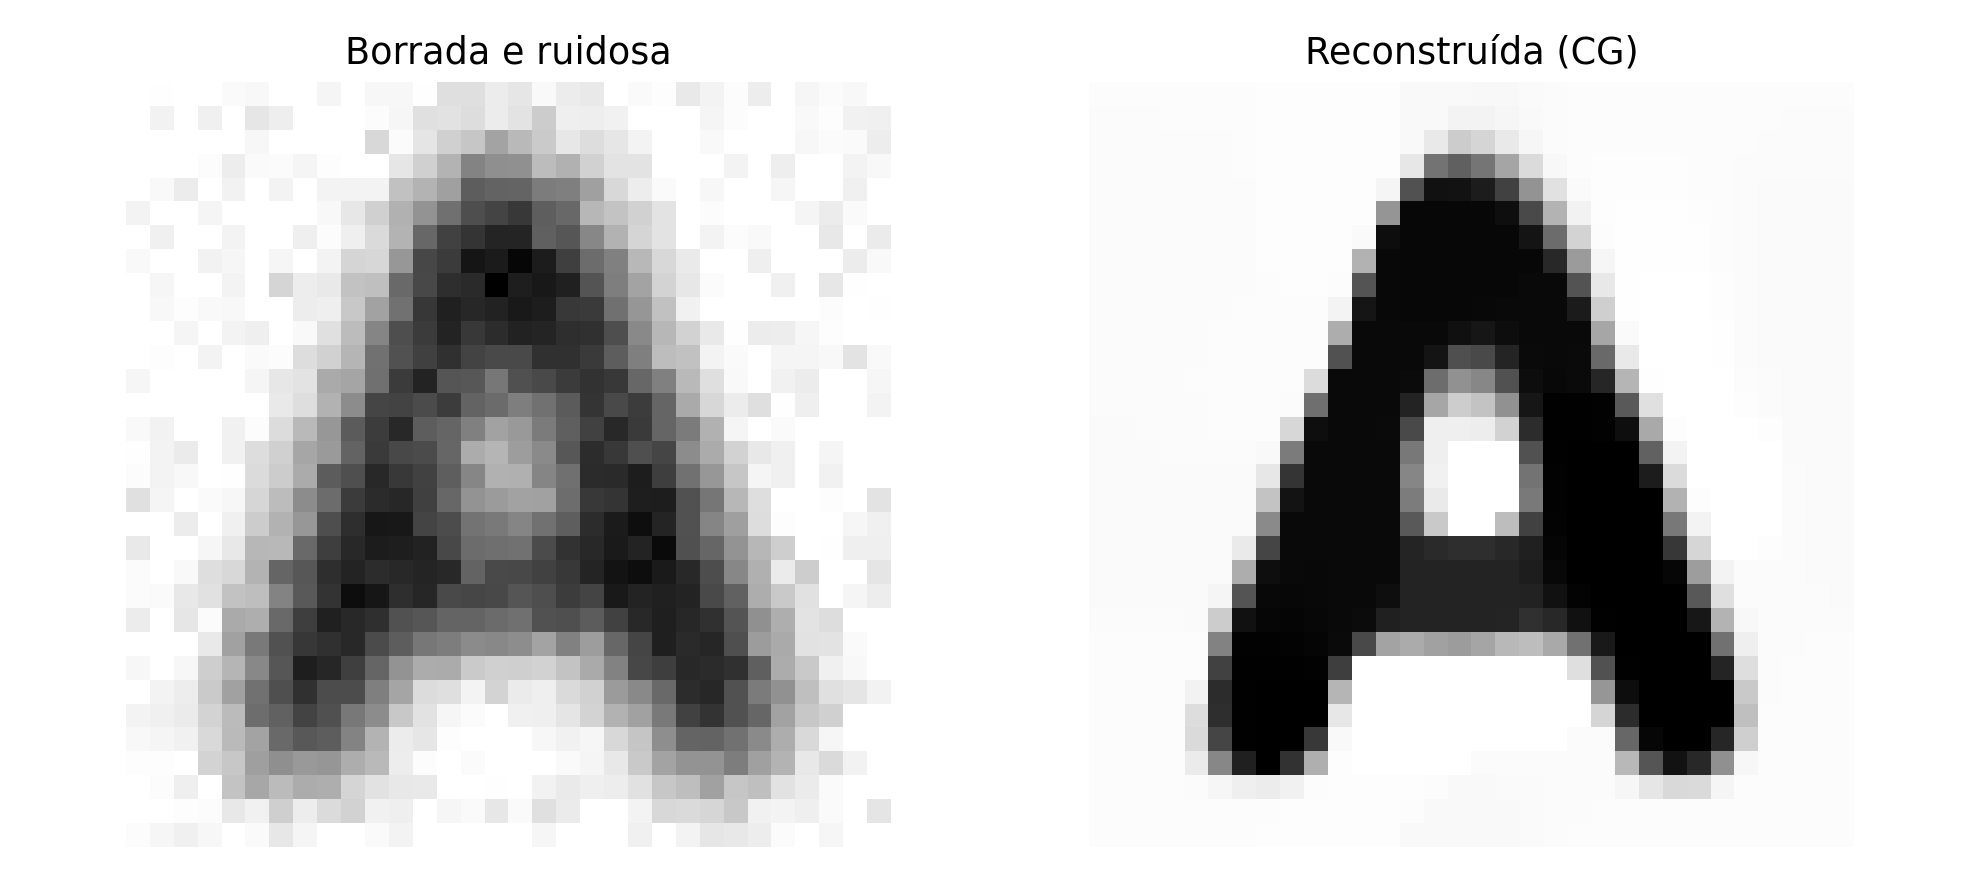
\includegraphics[width=0.75\textwidth]{questao2/comparacao_imagens.png}
\caption{Problema 2. Imagem borrada e ruidosa $b$ (esquerda) e imagem reconstruída pelo CG após 1000 iterações (direita).}
\label{fig:q2img}
\end{figure}

\begin{figure}[H]
\centering
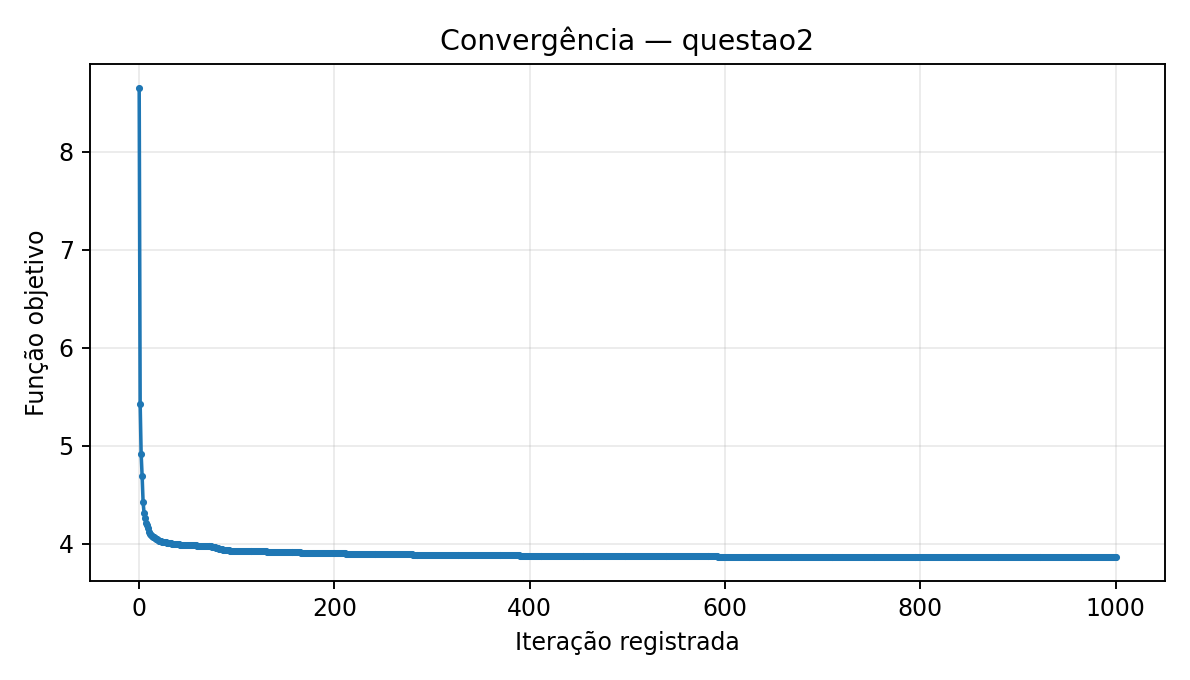
\includegraphics[width=0.65\textwidth]{questao2/convergencia.png}
\caption{Problema 2. Valor de $f$ por iteração do CG.}
\label{fig:q2conv}
\end{figure}

\subsection{Discussão}

O CG reduziu a função-objetivo em cerca de 55\% ($8{,}65 \to 3{,}86$). A maior parte da redução veio do termo de fidelidade ($6{,}45\to1{,}74$): ao contrário de $b$, que é a imagem borrada, a reconstrução $x$ é tal que $Ax$ (a reconstrução borrada) se aproxima de $b$. O termo TV também diminuiu levemente ($110{,}0\to105{,}9$), refletindo a remoção do ruído nas regiões de fundo.

Visualmente (Figura~\ref{fig:q2img}), a reconstrução é muito mais nítida que a imagem degradada: a letra ``A'' tem bordas bem definidas, o fundo ficou praticamente uniforme e a abertura interna da letra é claramente visível. Esse é o comportamento esperado da regularização por variação total, que favorece imagens constantes por partes e preserva bordas.

Quanto à convergência (Figura~\ref{fig:q2conv}), a função cai rapidamente nas primeiras iterações ($f=4{,}12$ após 10 iterações e $3{,}93$ após 100) e depois decresce muito lentamente: entre as iterações 100 e 1000 a redução é de menos de 2\%. O algoritmo parou pelo limite de 1000 iterações, sem atingir a tolerância de gradiente ($\|\nabla f\|\approx0{,}049 > 10^{-5}$); ou seja, o ótimo não foi atingido com alta precisão. Esse comportamento é coerente com o mau condicionamento causado pelo $\epsilon$ pequeno na TV: o CG avança rapidamente nas direções bem condicionadas e lentamente nas demais.

Por fim, como o problema é irrestrito, não se impôs que os pixels ficassem em $[0,1]$: a reconstrução tem valores entre $-0{,}031$ e $1{,}028$ (36 pixels abaixo de 0 e 68 acima de 1). As violações são pequenas e a figura usa a escala visual $[0,1]$.

% =====================================================================
\section{Problema 3 --- Precificação minimax}

\subsection{Análise da função-objetivo}

A função a minimizar é
\begin{equation}
F(p_1,p_2) = \max_{i=1,\dots,4} \left|\frac{a_{1,i}}{p_1}+\frac{a_{2,i}}{p_2} - R_{\mathrm{alvo}}\right|, \qquad p_1,p_2>0,
\end{equation}
com $R_{\mathrm{alvo}}=10000$ e os parâmetros da Tabela~1 do enunciado. Suas características são:

\begin{itemize}
  \item \textbf{Dimensão.} Apenas 2 variáveis, restritas a valores positivos.
  \item \textbf{Não diferenciabilidade.} O valor absoluto não é diferenciável onde o desvio de um cenário se anula, e o máximo não é diferenciável onde dois cenários empatam como pior caso. A função é contínua mas apresenta ``quinas''. Em problemas minimax, o ótimo tipicamente fica \emph{exatamente} em uma dessas quinas, pois a solução equilibra os piores desvios.
  \item \textbf{Convexidade.} Com a troca $u=1/p_1$, $v=1/p_2$, cada receita é linear em $(u,v)$ e $F$ torna-se o máximo de valores absolutos de funções afins, ou seja, uma função convexa e linear por partes em $(u,v)$. Como cada preço corresponde a um único par $(u,v)$ e vice-versa, um mínimo local nos preços também é mínimo local em $(u,v)$ e, pela convexidade, é global. Assim, $F$ não tem mínimos locais ``falsos'', mesmo não sendo convexa nos preços.
  \item \textbf{Estrutura dos cenários.} Os cenários 1, 2 e 3 são proporcionais: os cenários 2 e 3 valem $0{,}7$ e $1{,}3$ vezes o cenário 1. Definindo $s = 100000/p_1 + 80000/p_2$, tem-se $R_1=s$, $R_2=0{,}7s$ e $R_3=1{,}3s$. Se $s\ge R_{\mathrm{alvo}}$, então $|R_3-R_{\mathrm{alvo}}|\ge 0{,}3R_{\mathrm{alvo}}$; se $s\le R_{\mathrm{alvo}}$, então $|R_2-R_{\mathrm{alvo}}|\ge 0{,}3R_{\mathrm{alvo}}$. Logo $F\ge 3000$ em todo o domínio, com igualdade quando $s=R_{\mathrm{alvo}}$ e o cenário 4 não excede esse desvio. Sobre a curva $s=R_{\mathrm{alvo}}$ verifica-se que $R_4\in(9000,\,11250)$, de modo que o cenário 4 nunca é o pior. Assim, \textbf{o valor ótimo é 3000 e o conjunto de ótimos é a curva}
  \begin{equation}
  \frac{100000}{p_1}+\frac{80000}{p_2} = 10000, \qquad p_1>10,\ p_2>8,
  \end{equation}
  e não um ponto isolado.
\end{itemize}

\subsection{Escolha do método: Nelder--Mead Simplex}

\begin{itemize}
  \item Métodos baseados em gradiente (gradiente descendente, BFGS, CG, Newton) pressupõem uma função diferenciável. Aqui o gradiente não existe justamente no ótimo, a busca linear tende a falhar nas quinas e as aproximações de Hessiana do BFGS perdem o sentido.
  \item O \textbf{Nelder--Mead} usa apenas valores da função, sem derivadas, e por isso não é afetado pelas quinas.
  \item Com apenas 2 variáveis, o simplex tem 3 vértices e o custo por iteração é desprezível. A ausência de garantias gerais de convergência do Nelder--Mead não é preocupante aqui, pois o resultado pode ser verificado pelo limitante inferior $F\ge3000$ deduzido acima.
\end{itemize}

Para manter os preços estritamente positivos sem impor restrições, otimizou-se nas variáveis $z_j=\ln p_j$, isto é, $p_j=e^{z_j}$. Trata-se apenas de uma mudança de variáveis; o algoritmo de otimização continua sendo o Nelder--Mead irrestrito.

\subsection{Resultados}

Utilizou-se \texttt{method='Nelder-Mead'} com ponto inicial $p_0=(12,\,25)$, \texttt{xatol}$=10^{-12}$ e \texttt{fatol}$=10^{-9}$. Os resultados estão na Tabela~\ref{tab:q3}.

\begin{table}[H]
\centering
\caption{Resultados do Problema 3 (Nelder--Mead).}
\label{tab:q3}
\begin{tabular}{@{}lcc@{}}
\toprule
Cenário & Receita $R_i$ & Desvio $|R_i-R_{\mathrm{alvo}}|$ \\
\midrule
1 --- Mercado Normal      & $10000{,}0$ & $0{,}0$ \\
2 --- Recessão Econômica  & $7000{,}0$  & $3000{,}0$ \\
3 --- Alta Demanda        & $13000{,}0$ & $3000{,}0$ \\
4 --- Pressão Competitiva & $9770{,}2$  & $229{,}8$ \\
\midrule
Preços ótimos $(p_1,p_2)$ & \multicolumn{2}{c}{$(15{,}204;\ 23{,}372)$} \\
Pior desvio $F(p^*)$ & \multicolumn{2}{c}{$3000{,}0$} \\
Iterações / avaliações de $F$ & \multicolumn{2}{c}{116 / 250} \\
\bottomrule
\end{tabular}
\end{table}

\begin{figure}[H]
\centering
\begin{minipage}{0.49\textwidth}\centering
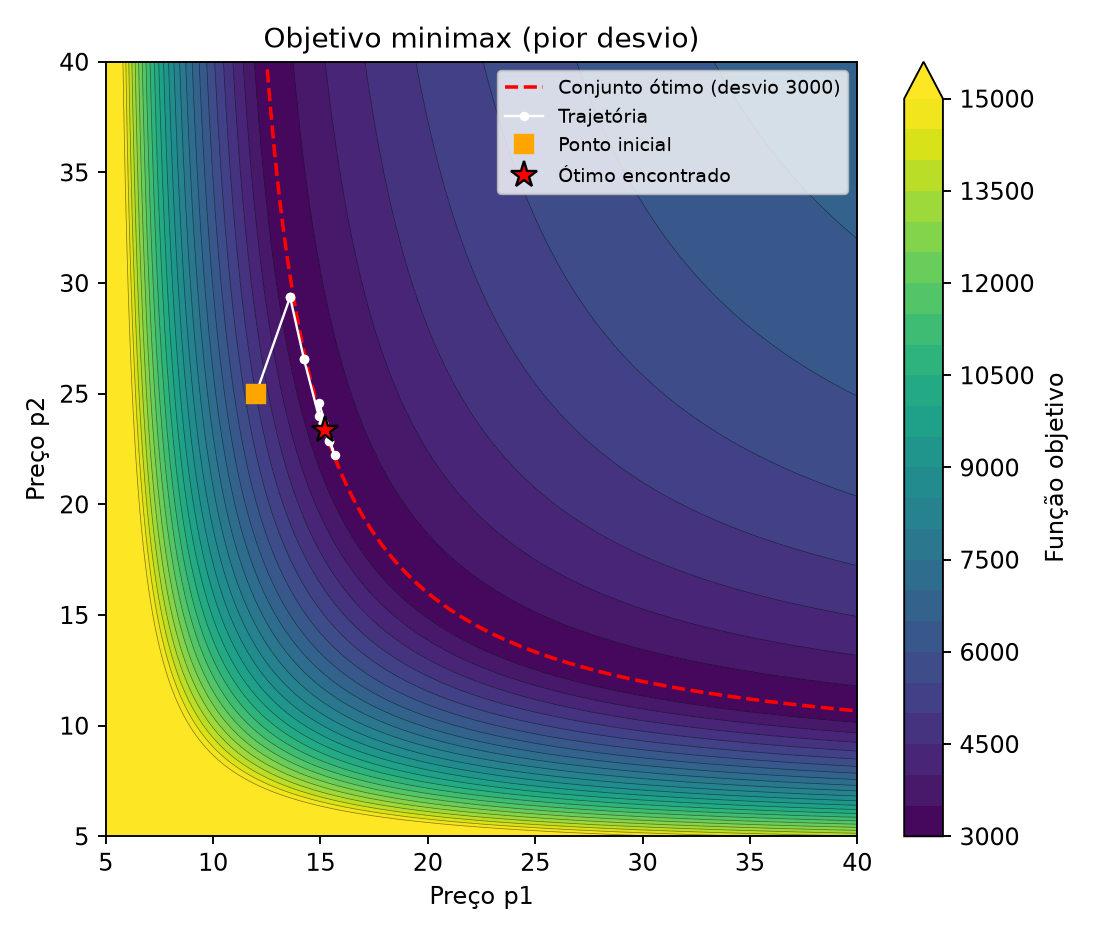
\includegraphics[width=\linewidth]{questao3/contorno.png}
\end{minipage}\hfill
\begin{minipage}{0.49\textwidth}\centering
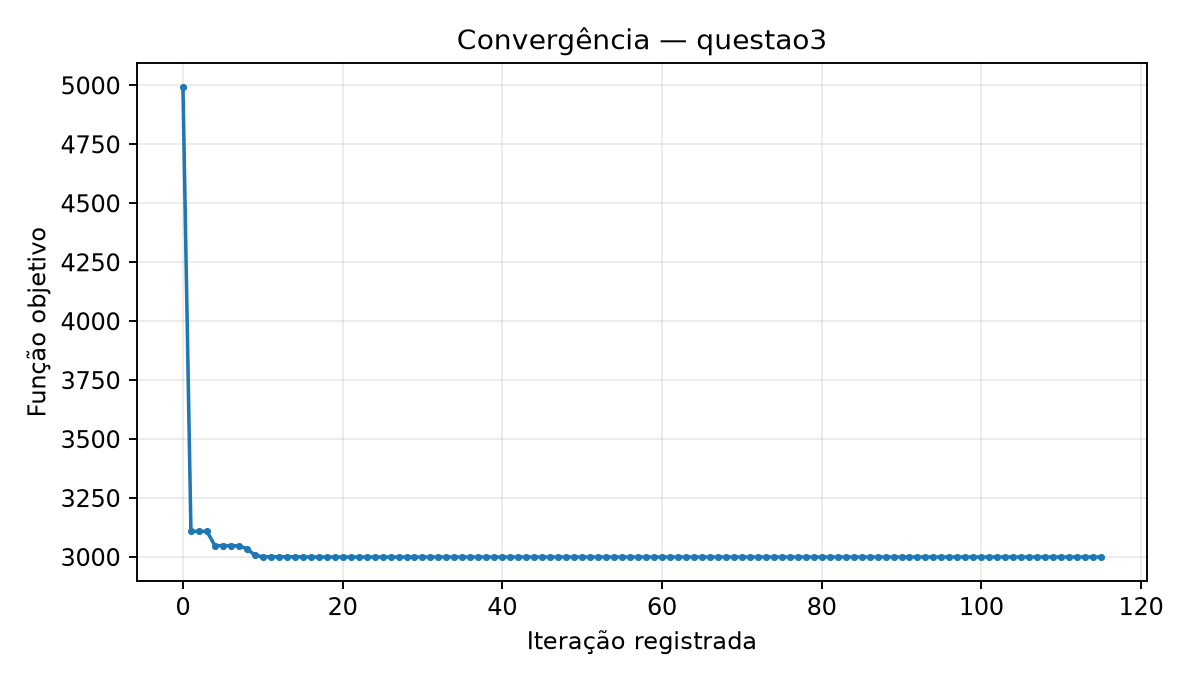
\includegraphics[width=\linewidth]{questao3/convergencia.png}
\end{minipage}
\caption{Problema 3. Esquerda: curvas de nível do pior desvio, com a trajetória do Nelder--Mead e a curva de ótimos (tracejada). Direita: pior desvio por iteração.}
\label{fig:q3}
\end{figure}

\subsection{Discussão}

O Nelder--Mead atingiu o valor ótimo $F=3000$, que coincide com o limitante inferior obtido analiticamente. A solução encontrada satisfaz $R_1 = 10000$, ou seja, está exatamente sobre a curva de ótimos, e nela os cenários 2 (Recessão) e 3 (Alta Demanda) empatam como pior caso, com desvios de $3000$ para baixo e para cima, respectivamente. Esse empate é a ``quina'' em que se encontra o ótimo, confirmando que a função não é diferenciável na solução. O cenário 4 fica bem abaixo do pior caso (desvio de 230).

A Figura~\ref{fig:q3} mostra que o pior desvio cai de 4993 para cerca de 3001 em aproximadamente 10 iterações; as iterações restantes apenas contraem o simplex até as tolerâncias muito pequenas adotadas. No gráfico de curvas de nível, a região de valor mínimo forma um vale estreito ao longo da curva tracejada, e a trajetória termina sobre ela.

Uma consequência importante da análise é que \textbf{os preços ótimos não são únicos}: qualquer par $(p_1,p_2)$ sobre a curva $100000/p_1+80000/p_2=10000$ garante o mesmo pior desvio de 3000. Os preços $(15{,}20;\ 23{,}37)$ reportados são apenas o ponto da curva ao qual o Nelder--Mead chegou a partir de $p_0=(12,25)$; outro ponto inicial levaria, em geral, a outro par de preços com o mesmo valor ótimo. Na prática, a empresa pode escolher qualquer ponto dessa curva usando um critério adicional (por exemplo, a receita no cenário 4 ou restrições comerciais sobre os preços).

% =====================================================================
\section{Problema 4 --- Equilíbrio do sistema de carrinhos}

\subsection{Análise da função-objetivo}

A energia potencial é
\begin{equation}
U(x_1,x_2) = \tfrac12 k_2x_1^2 + \tfrac12 k_3(x_2-x_1)^2 + \tfrac12 k_1x_2^2 - Px_2,
\end{equation}
que pode ser escrita como uma forma quadrática
\begin{equation}
U(\mathbf{x}) = \tfrac12\mathbf{x}^T\mathbf{H}\mathbf{x} - \mathbf{c}^T\mathbf{x}, \qquad
\mathbf{H} = \begin{bmatrix} k_2+k_3 & -k_3\\ -k_3 & k_1+k_3\end{bmatrix} = \begin{bmatrix} 3500 & -2000\\ -2000 & 3000\end{bmatrix}, \qquad
\mathbf{c} = \begin{bmatrix}0\\P\end{bmatrix}.
\end{equation}

\begin{itemize}
  \item \textbf{Diferenciabilidade.} $U$ é um polinômio de grau 2, portanto infinitamente diferenciável, com gradiente $\nabla U = \mathbf{H}\mathbf{x}-\mathbf{c}$ e Hessiana constante $\mathbf{H}$.
  \item \textbf{Convexidade.} $\det\mathbf{H} = 6{,}5\times10^6>0$ e $\operatorname{tr}\mathbf{H}>0$, logo $\mathbf{H}$ é definida positiva (autovalores $1234{,}4$ e $5265{,}6$). A função é \emph{estritamente convexa} e possui um único mínimo global.
  \item \textbf{Condicionamento.} O número de condição de $\mathbf{H}$ é $5265{,}6/1234{,}4\approx4{,}3$, moderado. As curvas de nível são elipses inclinadas, pois $\mathbf{H}$ acopla $x_1$ e $x_2$.
\end{itemize}

\subsection{Escolha do método: Newton}

O método de Newton aproxima a função, a cada iteração, por seu modelo quadrático de segunda ordem e salta para o mínimo desse modelo. Como $U$ \emph{já é} quadrática, o modelo é exato e o primeiro passo
\begin{equation}
\mathbf{x}_1 = \mathbf{x}_0 - \mathbf{H}^{-1}\nabla U(\mathbf{x}_0) = \mathbf{H}^{-1}\mathbf{c}
\end{equation}
leva ao ótimo a partir de qualquer ponto inicial. Além disso, a Hessiana é constante, conhecida analiticamente e definida positiva, de modo que usá-la não tem custo extra nem risco de direção de subida. Nenhum outro método estudado converge em menos iterações para este problema.

Como a SciPy não oferece o método de Newton puro, usou-se \texttt{method='Newton-CG'} com gradiente e Hessiana analíticos. Esse método resolve o sistema de Newton $\mathbf{H}\mathbf{d}=-\nabla U$ por gradientes conjugados internos, o que, para um sistema $2\times2$ definido positivo, é exato em no máximo 2 passos internos; na prática, equivale ao Newton.

\subsection{Resultados}

Com ponto inicial $\mathbf{x}_0=(0,0)$ e \texttt{xtol}$=10^{-12}$, obtiveram-se os resultados da Tabela~\ref{tab:q4}.

\begin{table}[H]
\centering
\caption{Resultados do Problema 4 (Newton).}
\label{tab:q4}
\begin{tabular}{@{}ll@{}}
\toprule
Grandeza & Valor \\
\midrule
$x_1^*$ & $0{,}030769$ m ($=2/65$) \\
$x_2^*$ & $0{,}053846$ m ($=3{,}5/65$) \\
$U(\mathbf{x}^*)$ & $-2{,}6923$ J \\
Iterações & 2 \\
Avaliações de $f$ / de $\nabla f$ & 2 / 2 \\
Erro em relação à solução analítica $\mathbf{H}^{-1}\mathbf{c}$ & $6{,}9\times10^{-18}$ \\
$\|\nabla U(\mathbf{x}^*)\|$ & $1{,}7\times10^{-14}$ \\
\bottomrule
\end{tabular}
\end{table}

\begin{figure}[H]
\centering
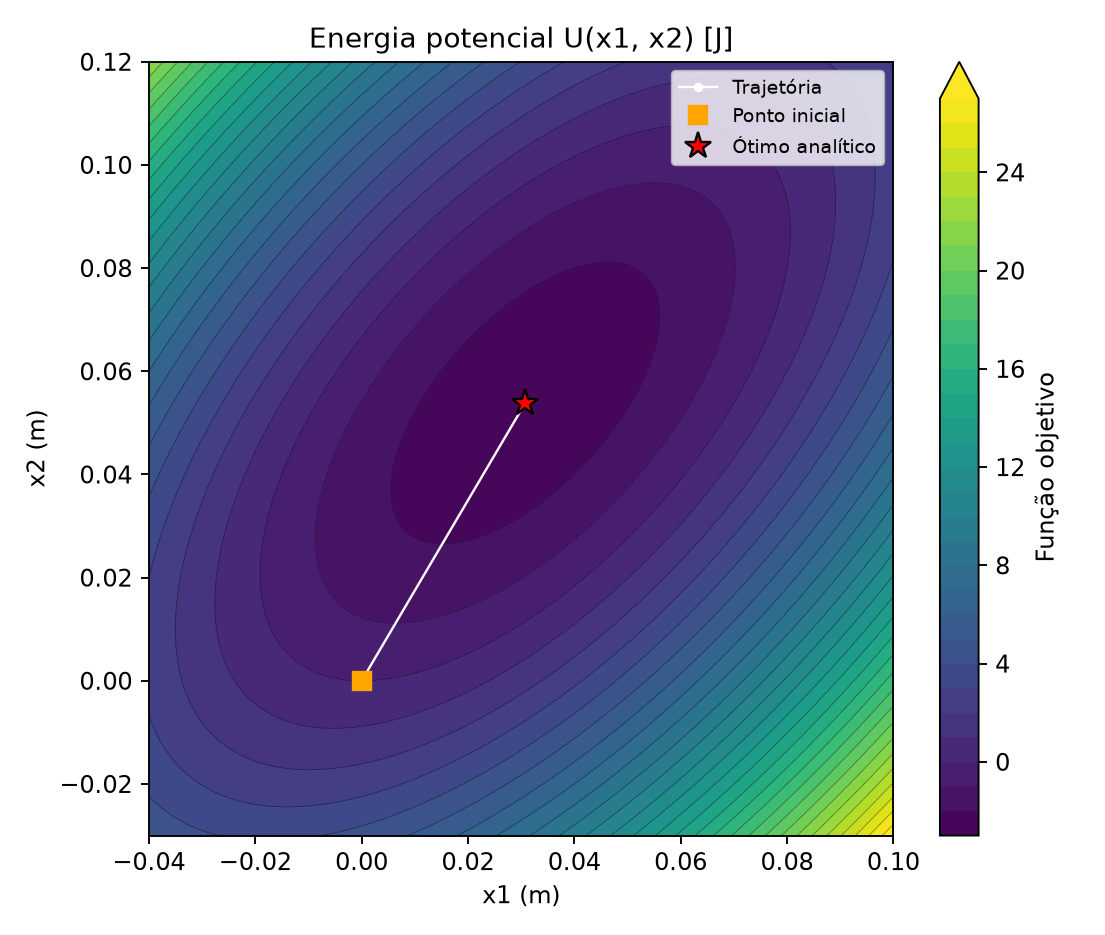
\includegraphics[width=0.6\textwidth]{questao4/curvas_nivel.png}
\caption{Problema 4. Curvas de nível da energia potencial $U$, com a trajetória do método de Newton a partir de $\mathbf{x}_0=(0,0)$.}
\label{fig:q4}
\end{figure}

\subsection{Discussão}

A posição de equilíbrio é $x_1^*\approx30{,}8$~mm e $x_2^*\approx53{,}8$~mm, idêntica à solução analítica de $\mathbf{H}\mathbf{x}=\mathbf{c}$ até a precisão de máquina. A energia potencial mínima é $U^*=-2{,}692$~J, que satisfaz a relação $U^* = -\tfrac12 P x_2^*$ válida no equilíbrio de sistemas lineares. Fisicamente, ambos os carrinhos se deslocam no sentido da força $P$, com $x_2^*>x_1^*$: o carrinho B, onde a força é aplicada, desloca-se mais, e a mola $k_3$ fica esticada, transmitindo parte da força ao carrinho A.

A Figura~\ref{fig:q4} ilustra a análise: as curvas de nível são elipses concêntricas em torno de um único ponto (convexidade estrita), e o Newton vai de $(0,0)$ ao ótimo em um único passo retilíneo. A SciPy reporta 2 iterações porque, após o primeiro passo já atingir o ótimo ($U$ passa de $0$ para $-2{,}6923$), uma segunda iteração com passo desprezível é executada antes de o critério de parada \texttt{xtol} ser satisfeito; o valor de $U$ não se altera nessa segunda iteração. O resultado confirma que, para funções quadráticas estritamente convexas, o método de Newton converge em uma iteração.

% =====================================================================
\section*{Conclusões}

A escolha do método em cada problema seguiu o mesmo critério: usar a maior quantidade de informação de derivadas que a função permite, desde que o custo computacional seja viável.

\begin{itemize}
  \item No \textbf{Problema 4}, a função é quadrática com Hessiana constante e definida positiva, e o \textbf{método de Newton} converge em uma única iteração.
  \item No \textbf{Problema 1}, a função é suave mas tem Hessiana singular no ótimo e indefinida fora dele; o \textbf{BFGS}, com aproximação definida positiva da Hessiana, convergiu superlinearmente em 7 iterações para o menor autovalor de $\mathbf{K}$, com $\omega_1\approx0{,}445$~rad/s.
  \item No \textbf{Problema 2}, a dimensão elevada ($n=1024$) torna inviável o uso de Hessianas; os \textbf{Gradientes Conjugados}, com memória $O(n)$, recuperaram uma imagem nítida, embora o mau condicionamento introduzido pelo $\epsilon$ da variação total tenha impedido a convergência com alta precisão dentro de 1000 iterações.
  \item No \textbf{Problema 3}, a função minimax não é diferenciável no ótimo, e o \textbf{Nelder--Mead}, que não usa derivadas, atingiu o pior desvio mínimo de 3000. A análise mostrou ainda que existe uma curva inteira de preços ótimos.
\end{itemize}

Em todos os casos os resultados numéricos foram validados de forma independente: por autovalores (Problema 1), por diferenças finitas do gradiente (Problema 2), por um limitante inferior analítico (Problema 3) e pela solução de um sistema linear (Problema 4).

\section*{Códigos-fonte}

Os códigos acompanham este relatório: \texttt{questao1.py} a \texttt{questao4.py} (um por problema), \texttt{comum.py} (exportação dos resultados e geração de gráficos) e \texttt{utils.py} (leitura da imagem e operador de borrão, fornecidos com o enunciado). Para reproduzir os resultados, basta instalar as dependências com \texttt{pip install -r requirements.txt} e executar cada script a partir da pasta do projeto.

\end{document}
